% !TeX spellcheck = en_US
\documentclass[french]{yLectureNote}

\title{Optique ondulatoire}
\subtitle{Physique}
\author{Paulhenry Saux}
\date{\today}
\yLanguage{Français}

\professor{F.Pettinari}
\usepackage{graphicx}%----pour mettre des images
\usepackage[utf8]{inputenc}%---encodage
\usepackage{geometry}%---pour modifier les tailles et mettre a4paper
%\usepackage{awesomebox}%---pour les boites d'exercices, de pbq et de croquis ---d\'esactiv\'e pour les TP de PC
\usepackage{tikz}%---pour deiffner + d\'ependance de chemfig
% \usepackage{tabularx}%---pour dimensionner automatiquement les tableaux avec variable X
\usepackage{awesomebox}%---Pour les boites info, danger et autres
\usepackage{menukeys}%---Pour deiffner les touches de Calculatrice
\usepackage{fancyhdr}%---pour les en-t\^ete personnalis\'ees
\usepackage{blindtext}%---pour les liens
\usepackage{hyperref}%---pour les liens (\`a mettre en dernier)
\usepackage{caption}%---pour la francisation de la l\'egende table vers Tableau
\usepackage{pifont}
\usepackage{array}%---pour les tableaux
\usepackage{lipsum}
\usepackage{yFlatTable}
\usepackage{multicol}
\newcommand{\Lim}[1]{\lim\limits_{\substack{#1}}\:}
\renewcommand{\vec}{\overrightarrow}
\newcommand{\N}[0]{\mathbb{N}}
\newcommand{\dd}{\mathrm{d}}
\newcommand{\norm}[1]{||\vec{#1}||}
\newcommand{\fo}{\psi(\vec{r},t)}
\newcommand{\foe}{\psi(\vec{r},t)\*}
\newcommand{\HH}{\hat{H}}
\newcommand{\hb}{\hbar}
\newcommand{\lap}{\nabla^2}
\newcommand{\lapcc}{\frac{\partial^2 }{\partial x^2}+\frac{\partial^2 }{\partial y^2}+\frac{\partial^2 }{\partial z^2}}
\newcommand{\mpsi}{\(\psi\)}
\newcommand{\und}{\underline}
\begin{document}
%Voir les notes de cours  à synthétiser
% Les rayons se propagent en ligne droite, sous les hypothèses :
% \begin{itemize}
%  \item milieu homogène
%  \item Diffraction négligée
%  \item Pas d'intéraction des rayons lumineux
% \end{itemize}
% Elles ont permis l'étude de la formtion d'image. L'Optique ondulatoire vise à comprendre les phénonèmes ondulatoires\marginCheck{Valable aussi pour d'autres ondes (son, onde gravitationnelle)}.
\chapter{Modèle scalaire}
\section{Fonction d'onde}
\begin{definition}[Lumière]
La lumière est une onde électromagnétique. Il y a donc 2 champs \(\vec{E}+\vec{B}\).
\end{definition}
Par l'approximation scalaire, on associe l'onde non plus à des fonctions vectorielles mais à une fonction scalaire \(\psi(M, t)\) dépendant de la position (\(\vec{OM} = \vec{r}\)) et du temps\marginCritical{On suppose donc que cette fonction d'onde de 4 variables décrit tous les phénomènes étudiés}.
% C'est un cas général d'un champ physique\marginCheck{Un champ est en effet une fonction dépendant de ces 4 variables définie partout}.

\begin{theorem}[Équation d'onde]
\[\lap \psi - \frac{1}{v^2} \frac{\partial ^2 \psi}{\partial t^2} = 0\] avec
\(v\) la vitesse de propagation de l'onde \(v = \frac{c}{n}\).
\end{theorem}
% \(\lap\) le laplacien \(\frac{\partial^2 \psi}{\partial x^2}+\frac{\partial^2 \psi}{\partial y^2}+\frac{\partial^2 \psi}{\partial z^2}\) et
\begin{definition}[Période d'oscillation]
L'oscillation de \(\psi\) en fonction du temps se fait à une période de \(T = \frac{\lambda}{v} \simeq 10^{-15}\)s.
\end{definition}
On obtient un ordre de grandeur de l'odre de la femtoseconde, qui est une grandeur impossible à mesurer. On mesure donc une intensité lumineuse en \(W/m^2\)
\marginTips{Une énergie arrivée pendant un certain temps sur une certaine surface.}.
\begin{definition}[Intensité lumineuse]
C'est ce qui est mesuré par les capteurs : \(I = \frac{E}{\Delta t \times S} \propto \fo^2\).
\end{definition}
% I est la moyenne temporelle de \(\fo^2\), i.e. \(I = 2<\fo^2>\). Avec une fonction complexe, on aura \(I = |\fo|^2\).
\section{Types d'onde}
\subsection{Onde progressive à une dimension}
\begin{definition}[Onde progressive]
Elle ``avance'' dans une direction à une vitesse v.
\end{definition}
\includegraphics[scale=0.5]{c1_s0}

Au temps \(t_1>t_0\), il y a une translation de \(\psi(x,t_0) = f(x)\) en \(t_1\) de façon à obtenir \(\psi(x,t_1) = f(x-vt_1)\)\marginCritical{Si on met un plus à la place du moins, il y a une propagation dans le sens des x décroissants au lieu des x croissants}.

On vérifie que cette solution vérifie l'équation :

\explanation{0}{On utilise la règle de la chaine pour les fonctions composées}

\explanation{c1}{On utilise deux fois la règle de la chaine pour les fonctions composées}
%TODO documenttation pour ce bug

\begin{flalign*}
\lap \psi &= \frac{\partial^2}{\partial x^2}(f(x-vt))\\
&= f''(x-vt)\explain{0}{right}{0}{0.5}{}\\
\frac{\partial^2\psi}{\partial t^2} &= \frac{\partial^2}{\partial t^2}f(x-vt)\\
    &= \frac{\partial}{\partial t}(f'(x-vt) \cdot (-v)) \\
    &= -v \frac{\partial}{\partial t}(f'(x-vt)) \\
    &= -v (f''(x-vt) \cdot (-v)) \\
    &= v^2 f''(x-vt)\explain{c1}{right}{0}{0.5}{}\\
&\lap \psi - \frac{1}{v^2}\frac{\partial^2 \psi}{\partial t^2} = 0
\end{flalign*}
\subsection{Ondes monochromatiques}
\begin{definition}[Onde monochromatique]
La dépendance temporelle est sinusoidale. On a alors \[\fo = A(\vec{r})\cos(\omega t+\varphi(\vec{r}))\]
\end{definition}
On reconnait l'amplitude de l'onde, \(\omega t + \varphi\) la phase en t quelconque, sans oublier \(\omega\) la pulsation de l'onde \(\frac{2\pi}{T}\).

On obtient alors l'équation de Helmotz : \[\lap \psi + \frac{\omega^2}{v^2}\psi = 0\]
\subsubsection{Intensité}
L'intensité vaut :

\explanation{c2}{En effet, la moyenne d'une fonction sinusoïdale ou cosinusoïdale sur un ou plusieurs cycles complets est nulle}

\begin{flalign*}
I(\vec{r}) &= 2 <A^2(\vec{r})\cos^2(\omega t + \varphi(\vec{r}))>\\
&= 2<A^2\frac12(1+\cos(2(\omega t + \varphi)))>\explain{c2}{right}{0}{0.5}{}\\
&= A^2
\end{flalign*}
L'intensité dépend donc de l'amplitude.
\subsubsection{Surface d'onde}
\begin{definition}[Surface d'onde]
Une surface telle que \(\varphi(\vec{r})\) est constant, ce qui implique que \(\cos()\) prend la m\^eme valeur pour un certin tempsf
\end{definition}
\subsection{Onde plane progressive monochromatique (OPPM)}
\subsubsection{Définitions}
\begin{definition}[Onde plane]
Les surfaces d'onde sont des plans qui avancent dans une direction à la vitesse v.
\end{definition}
\begin{definition}[OPPM]
Elle est de la forme \(\fo = A\cos(\omega t - \vec{k}\cdot \vec{r} + \varphi_0)\).
\end{definition}
%  On cherche donc A et \(\varphi\).
\begin{center}
\begin{tabular}{ll}
Propriété & Signification\\
Plane & Les surfaces d'onde sont des plans\\
Progressive & Elle se dirige dans une certaine direction à une vitesse de propagation\\
Monochromatique & La dépendance temporelle est sinusoidale.
\end{tabular}
\end{center}
\subsubsection{Propriétés}
% L'équation d'un plan est de la forme \(\alpha x + \beta y + \gamma z = C\) avec \(\vec{u}(\alpha, \beta, \gamma), \vec{r}(x,y,z)\). On peut donc la réécrire sous la forme \(\vec{u}\cdot \vec{r} = K\) avec \(\vec{u}\) un vecteur orthogonal au plan.

On prend \(\varphi(\vec{r}) =\vec{k}\cdot \vec{r}\)\marginTips{\(\vec{k}\) est le vecteur d'onde. Il donne la direction de propagation de l'onde. Il est donc dans la m\^eme direction que \(\vec{u}\). On remarque que la phase augmente comme \(\vec{k}\cdot \vec{r}\) augmente lors de la propagation.}
et A constant pour obtenir\marginInfo{Cette fonction est bien de la forme \(f(vt - x)\) avec \(x= \vec{u}\cdot \vec{r}, v=\omega\), donc elle est bien progressive. Elle respecte bien la condition d'une onde monochromatique \(\cos(\omega t + \varphi(\vec{r}))\), avec \(\varphi(\vec{r}) = \vec{k}\cdot\vec{r}+\varphi_0\)}
\[\fo = A\cos(\omega t - \vec{k}\cdot \vec{r} + \varphi_0)\]

% C'est bien une fonction d'onde. En effet, on peut la réecrire sous la forme \[\fo = A\cos(\omega(\frac{k_x}{\omega}x + \frac{k_y}{\omega}y + \frac{k_z}{\omega}z))\]
% et vérifier que cela vérifie l'équation
% \begin{flalign*}
% \frac{\partial^2 \psi}{\partial t^2} &= -\omega^2 \psi\\
% \lap \psi &= -k_x^2\psi -k_y^2\psi -k_z^2\psi\\
% &= -\norm{k}^2\psi\\
% 0 &= (-k^2 + \frac{\omega^2}{v^2})\psi
% \end{flalign*}

% On en déduit :
\begin{theorem}[Relation de dispersion]
\[\omega  = \frac{c}{n}\norm{k}\]
\end{theorem}

% Si \(\vec{k} = k \vec{e_z}\)\marginWarning{\(\vec{k}\) est le vecteur d'onde, il définit la direction de propagation.}, alors \(\fo = A\cos(\omega t - kz + \varphi_0)\) qui est périodique en T de période \(\frac{2\pi}{\omega}\) en z de période \(\frac{2\pi}{k} = \lambda\).

Avec la relation de dispersion, on obtient \(\lambda = \frac{\lambda_0}{n}\) avec \(\lambda_0 = \frac{2\pi c}{\omega}\)\marginCritical{La couleur n'est pas définie par \(\lambda\) mais pas \(\lambda_0\), i.e. la pulsation !}

% \warningInfo{Équivalence d'écriture}{On a \[\psi_0 \cos(\omega(t-\frac{\vec{k}\cdot \vec{r}}{\omega})+\varphi_0) = \psi_0 \cos(\omega(t-\frac{\vec{u}\cdot \vec{r}}{v})+\varphi_0)\] Le vecteur \(\vec{u}\) vaut alors \(\frac{\vec{k}}{\norm{k}}\)}
\warningInfo{Double périodicité}{Il ne faut pas confondre la périodicité spatiale \(\lambda  = \frac{2\pi}{k}\) et la périodicité temporelle \(T = \frac{2\pi}{\omega}\)}
\subsection{Onde sphérique monochromatique}

\subsubsection{Definition}
\begin{definition}[Onde sphérique]
Les surfaces d'onde sont des sphères concentriques. Elles sont de la forme \(\fo = \frac{A}{r} \cos(\omega t-kr)\)
\end{definition}
On en déduit que \(\varphi(\vec{r}) = \pm kr+\varphi_0\) avec r le rayon depuis l'origine.\marginTips{Cela signifie qu'à un instant t donné, on a la m\^eme phase d'onde sur des sphères concentriques séparés de \(\lambda\)}
\warningInfo{Convergence/Divergence}{Pour \(\cos(\omega t-kr)\), on est en présence d'une onde divergence, dans le cas contraire, \(\cos(\omega t + kr)\), c'est convergent.}
En effet, la surface d'onde a un rayon croissant au cours du temps (pour une phase donnée) avec une phase \(\omega t -kr\) et inversement.
\subsubsection{Vecteur d'onde}
Il vérifie toujours la realtion de dispersion.

Comme il n'y a plus de direction de propagation, on ne peut plus définir le vecteur d'onde. Cependant, l'onde converge/diverge  de l'origine. On peut donc prendre \(\vec{u} = \pm \vec{e_r}, \vec{k} = \pm k \vec{e_r}\) qui est valable pour tous les points de l'espace\marginCheck{En effet, \(\vec{k}\) est bien localement perpendicualire au surfaces d'onde en tout point.}.
\subsubsection{Amplitude}
Prenons l'onde divergente \(\fo = A(\vec{r})\cos(\omega t - kr)\). On sait que l'intensité est une puissance surfacique. Cela signifie que pour une m\^eme surface d'onde, la puissance totale doit toujours \^etre la m\^eme au cours de la propagation, et donc indépendante de \(r\).\marginInfo{En d'autres termes, cela signifie que l'amplitude dans une direction diminue avec la distance} On en déduit que \(A(\vec{r}) \propto \frac{1}{r}\):

% On a donc \[\fo = \frac{A}{r} \cos(\omega t-kr)\] et on remarque que l'onde n'est pas définie en 0 car \(A(\vec{r})\) diverge.\marginCritical{Les calculs précédents sont vrais pour une onde sphériqu isotopoe, avec A qui ne dépend pas de l'angle. }
\section{Lien avec l'optique géométrique}
\subsubsection{Notions élémentaires}
Un rayon lumineux correspond à un vecteur d'onde pris en un point de l'espace.

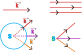
\includegraphics[scale=0.6]{c1_s2}
\subsubsection{Chemin optique et phase}
% \begin{definition}[Chemin optique]
% C'est \[\int_A^B\dd s n = n \times AB\] si propagation en ligne droite.
% \end{definition}
Le chemin optique est relié par la phase d'une onde se propageant entre les deux points. On a donc, à un instant donné :
\begin{flalign*}
\varphi_B-\varphi_A &= \vec{k}\cdot \vec{r_b} - \vec{k}\cdot \vec{r_a}\\
&= -\vec{k}\cdot(\vec{r_b}-\vec{r_a})\\
&= -\vec{k}\cdot \vec{AB}\\
&= \frac{n\omega}{c}AB\explain{c23}{right}{0}{0.5}{×}\\
&= \frac{2\pi}{\lambda} n \cdot AB
\end{flalign*}
\explanation{c23}{Le signe de k n'a pas d'importance car on cherche une différence de phase. On peut l'enlever, cela reste physiquement juste.}
\subsubsection{Théorème de Malus}
\begin{theorem}[Théorème de Malus]
 Les rayons lumineux sont orthogonaux aux surfaces d'onde en tout point.
\end{theorem}
\subsection{Notation complexe}
On remplace \(\fo\) par sa version complexe : \[\underline{\fo} = A(\vec{r}e^{-i(\omega t + \varphi(\vec{r}))})\] avec \(\fo = Re(\underline{\fo})\) et \(A(\vec{r}) = |\und{\fo}|\) et \(-(\omega t + \varphi(\vec{r})) = \arg(\und{\fo})\)

Pour une OPPM, on a \(\und{\fo} = Ae^{-i\varphi_0}e^{-i(\omega t-\vec{k}\cdot \vec{r})}\) avec \(Ae^{-i\varphi_0} = \und{A}\) l'amplitude complexe.

L'intensité se calcule avec \(I = |\und{\fo}|\)
 \end{document}
